\chapter{Memoria}
\minitoc{}
\section{Objeto}
El objeto de éste proyecto es la implementación de un sistema de \emph{Honeypots} utilizando \emph{containers}. 
Las Honeypots han existido desde hace bastante tiempo, quizá el software más conocido es honeyd, publicado en 2007.

\emph{Honeyd} (veasé \cite{honeynet-lowinteraction}) y otros casos son aplicaciones de las llamadas honeypots de baja interacción, puesto que sólo exponian al atacante un entorno limitado
no real y limitado frente a las \emph{honeypots} de alta interacción que permiten al atacante interactuar con la aplicación a investigar, el sistema operativo
y todo aquello que pueda ser relevante para la diagnosis como el trafico de red.

Habitualmente las \emph{honeypots} de alta interacción eran servidores fisicos o virtualizados creados exclusivamente para ésta tarea, lo que implica
una utilización de recursos en terminos de CPU, RAM (en definitiva en coste economico), considerando ademas que una honeypot por sus caracteristicas
y seguridad seguramente no se despliegue exactamente en el mismo entorno que el resto de aplicaciones de negocio de una organización, o en caso de hacerlo
la gestión del riesgo y medidas de seguridad aumentarian.

Por ello, desplegar y mantener honeypots de alta interacción es dificil. Desde la introducción de LXC (Linux Containers) en el kernel de Linux que los hizo posible, y
especialmente desde la aparición de Docker, que le dio popularidad y facilito su adopción y explotación.

Un \emph{container} es un metodo de virtualización para ejecutar multiples sistemas linux aislados (\emph{containers}) en un servidor que comparte un mismo kernel de Linux. Tecnicamente se basa en la utilización
de cgroups para limitar y priorizar recursos del sistema (CPU, memoria, I/O...) y de \emph{namespaces} que limitan la visualización del sistema de los procesos que se ejecutan en el \emph{container}, y es la tecnica que produce el aislamiento. Es importante notar que
frente a otras tecnologias de contanerización como \emph{Jails}, \emph{Zones} o incluso las maquinas virtuales, los \emph{containers} no tienen entidad propia para el kernel, asi que un \emph{container} se compone
de una definición de cgroup y namespace. 

Se puede considerar un container como un \emph{chroot} mejorado o como una maquina virtual ligera (que comparte el mismo kernel con el hipervisor), en éste sentido
mi interés en \emph{containers} para éste proyecto es debido a su eficiente utilización de recursos frente a una maquina virtual y a la facilidad
de crear, mantener y mejorar imagenes de sistema gracias al tooling alrededor de imagenes de Docker.

En resumen, el objeto de éste proyecto es el de construir una honeypot de alta interacción utilizando containers.

\section{Alcance}

El presente proyecto, tendrá como alcance:
\begin{itemize}
    \item La creación de una sonda que exponga al mundo el servicio que se quiere investigar que se ejecutará en un container.
    \item Las medidas de seguridad que se apliquen en dicha sonda.
    \item El uso de un sistema que guarde las trazas para poder identificar las acciones realizadas en la honeypot.
    \item El diseño de un sistema de colección, que recopile las trazas de las sondas y las almacene.
    \item el diseño de un sistema de explotación de datos de dicha colección, en particular la extracción, transformación y visualización de los mismos.
\end{itemize}

\section{Antecedentes}

% honeypots existentes...
% Kippo, honeyd, honeynet, dionaea 

El objetivo de una honeypot es el de aprender y conocer tecnicas de los atacantes para poder defenderse aplicando medidas de seguridad.
Debido al coste y complejidad de las honeypots de alta interacción, la mayoria de ellas son de baja interacción. Examinaré algunas de ellas:

\begin{enumerate}
    \item[\emph{Kippo}] (\cite{honeynet-kippo}) una honeypot de SSH de baja interacción, implementa el protocolo SSH en un servidor en Python
    lo que le permite extraer información del atacante (contraseña, IP, ordenes ejecutadas...), aunque intenta simular un servidor de SSH real
    se puede diagnosticar que el servidor es una honeypot simplemente ejecutando ordenes de sistema.
    \item[\emph{Dionaea}] (\cite{honeynet-dionaea}) una honeypot de baja interacción que simula varias aplicaciones como servidores TFTP, MySQL, HTTP, Memcache etc y expone sus puertos.
    \item[\emph{honeyd}] (\cite{honeynet-lowinteraction}) una de las primeras honeypots open source de baja interacción, puede exponer varios servicios aunque su desarrollo no está activo.
    \item[\emph{Dockerpot}] (\cite{honeynet-dockpot}) Una honeypot de alta interacción, basada en containers Docker, persigue un objetivo similar al de éste proyecto
    sin embargo no se expone directamente un container, se expone un proxy (a lo \emph{kippo}) que implementa el protocolo SSH, pero a diferencia de \emph{kippo} se abre otra conexion
    a un servidor SSH real que se ejecuta en un container. El proxy se encarga de levantar/parar el container, sólo se para el container cuando no hay ninguna conexión activa. Si el container es comprometido, siguiendo éste enfoque no se parará.
    De manera similar a \emph{Kippo} es fácil descubrir  que se esta atacando una honeypot de éste tipo, ya que la latencia entre que se inicia la comunicación
    y se pide la contraseña o se deniega el acceso al servidor SSH es sensiblemente elevada.
\end{enumerate}

Si hay algo en comun a todas ellas que motivó la creación de éste proyecto es que o bien son honeypots de baja interacción que son facilmente reconocibles
y por tanto carecen de interes para ataques reales o son de alta interacción pero para reciclar gestionar el servicio expuesto siempre hay un proxy delante
que se encarga de levantar / parar el container.

\nocite{*}
\nopagebreak
\printbibheading[title={Normas y referencias},heading=subbibnumbered]
\subsection{Disposiciones legales y normas aplicadas}
\subsubsection{Licencia FDL aplicable a ésta memoria}
\input{./fdl.tex}
\subsubsection{Licencia Apache 2.0 aplicable a todo el código fuente}
Todo el codigo fuente listado en ésta memoria o en soporte digital anexo se licencia bajo Apache License 2.0, una licencia libre sin \emph{copyleft} compatible con la GPL.
Se puede consultar los terminos de la licencia en la página de Apache \url{http://www.apache.org/licenses/LICENSE-2.0}

\subsection{Bibliografia}
\printbibliography[title={Referencias},heading=none]
\nopagebreak
\section{Definiciones y abreviaturas}
\section{Requisitos de diseño}

Para el diseño de la honeypot basada en containers hay que combinar principalmente funcionalidad, seguridad y viabilidad economica.

\begin{enumerate}
    \item[Flexible] la honeypot debe ser capaz de exponer cualquier tipo de servicio.
    \item[Eficiente] las sondas y el \emph{backend} deben minimizar el numero de servidores necesarios para su explotación.
    \item[Útil] Las honeypots deben exportar información útil.
    \item[Segura] las honeypots y el \emph{backend} deben proveer medidas de contencion frente atacantes.  
\end{enumerate}


\section{Análisis de soluciones para la sonda}

Lo más relevante de la sonda es la capacidad de extraer información de ella, a nivel de instrumentación. Cada proceso (y cabe recordar que un container en Linux es un proceso dentro de un \emph{namespace} con un \emph{cgroup} asociado) es gestionado, controlado
y auditado por el kernel.

Por ello, es interesante explorar si a través de alguna interfaz del kernel es posible instrumentar nuestra \emph{honeypot}. A la hora de exponer nuestro servicio, lo haremos utilizando
un container. existen diversas tecnologias para utilizar containers en Linux, de más a menos antiguedad se puede utilizar LXC, \emph{Docker}, \emph{LXD} ó \emph{rkt}.

\emph{LXC}, \emph{LXD} y \emph{rkt} comparten que su objetivo es el de proporcionar una \emph{lightweight-VM}, un entorno donde se pueden lanzar varios procesos y aplicaciones a la VM
pero sin la necesidad de cargar un kernel independiente y los costes extra que una VM supone (y perdiendo las garantias de aislamiento que también provee).

Docker, sin embargo, promueve una filosofia en la que cada container deberia albergar idealmente un sólo proceso o una aplicación.

Hay varias diferencias entre estas alternativas, \emph{LXC} y \emph{LXD} proveen herramientas para crear un container "manualmente" entrando en el container y lanzando los procesos. Mientras que Docker y rkt
lanzan containers utilizando imagenes. Una imagen no es mas que una descripción en un lenguaje de que contendrá el container, ordenes a lanzar para construir el container y el punto de entrada (la orden que se lanzara al lanzar el container) del mismo.

Los \emph{containers} construidos con \emph{Docker} y rkt son inmutables, cada imágen define varias capas de almacenamiento (veasé \cite{docker-storage}) que se van apilando
para construir el sistema de archivos, como ultima capa se añade una capa con permisos de lectura/escritura para permitir el almacenamiento temporal necesario para lanzar
la mayoría de ordenes.

Aunque cualquiera de las tecnologias de containerizacion explicadas previamente podrian ser utilizadas para nuestros fines, Docker tiene una amplia acogida como la herramienta de containerizacion
y hay muchisimas herramientas disponibles que suponen la utilización de Docker. Por ello, se escoge ésta tecnologia para construir nuestros containers.

\subsection{Instrumentación de los containers}

Cuando se habla de instrumentación de procesos en Linux, generalmente lo que queremos es obtener información de:
\begin{enumerate}
    \item[\emph{System calls}] Peticiones que realiza nuestro proceso al kernel (leer un fichero, abrir una conexión \ldots).
    \item[\emph{kernel function calls}] Que funciones se llamaran en el kernel para satisfacer una \emph{syscall}.
    \item[\emph{eventos}] eventos que se han definido en \emph{userspace} o dentro del kernel
\end{enumerate}

Para obtener ésta información hay diversas fuentes dentro del kernel:

\begin{enumerate}
    \item[\emph{kprobes}] el kernel modifica las instrucciones en ensamblador en tiempo de ejecución para activar la instrumentación. Si hablamos
    de \emph{kprobes} las funciones a instrumentar son parte del kernel. 
    \item[\emph{uprobes}] Similar a \emph{kprobes} pero para funciones en espacio de usuario como \emph{malloc}.
    \item[\emph{tracepoints}] A diferencia de un \emph{kprobe} o \emph{uprobe}, un tracepoint se define en el codigo fuente y se genera en tiempo de compilación, pudiendo ser activados en tiempo de ejecución cuando se requiera y extraer la información de ese \emph{tracepoint}.
    \item[\emph{ptrace}] A traves de la \emph{syscall ptrace (process trace)}, se le otorga a un proceso la capacidad de inspeccionar y modificar el comportamiento del proceso instrumentado. 
\end{enumerate}

Lo que se persigue en éste proyecto es intentar obtener la máxima información modificando lo minimo posible la aplicación instrumentada. Sería posible
reescribir el servicio expuesto implementando tracepoints para obtener información precisa, pero eso provocaria que la aplicación expuesta no fuese exactamente la misma que se utilizac
en otros entornos productivos (por lo que la información que nos provee podría ser inutil) ó aumentariamos la superficie de ataque, ya que estariamos
generando una versión nueva del \emph{software} que no está pasando quizá los mismos controles que el software original, y en cualquier caso, la modificación de todas las aplicaciones
que nos interesa analizar supone una inversión de esfuerzo que no es trivial.

No es interesante para éste proyecto información relativa al rendimiento, lo que sí nos intesa es información relativa al comportamiento de nuestra aplicación. Por lo tanto,
utilidades como \emph{perf} no nos seran utiles y se expondran alternativas a continuación.

\subsection{Obteniendo información del kernel: Auditd}

\emph{Audit} (veasé \cite{redhat-auditd}) es un subsistema del kernel y un conjunto de utilidades, 
disponibles desde el kernel 2.6 que nos proporcione información acerca de que \emph{syscalls}
se llaman desde los procesos del sistema. 
Es un componente maduro que se utiliza extensivamente (como prueba es parte de las recomendaciones del CIS y NIST para guias de bastionado)
y en base a un fichero de configuración se pueden definir que syscalls se monitorizaran
\emph{audit} genera un fichero de log que puede guardarse en disco, enviar eventos a un recolector remoto o ser expuesto via una conexión
\emph{netlink} (veasé \cite{wiki-netlink})

La primera aproximación realizada para la instrumentación de la sonda, fue utilizando \emph{auditd} es tan simple como lanzar un \emph{container} exponiendo un servicio
y guardar cualquier syscall recibida. 

Este enfoque puede ser costoso a nivel de rendimiento, depende del número de eventos generados (tráfico / operaciones del container) a la hora de la colección de eventos
y costoso también a la hora de extraer información relevante.

La idea inicial es configurar \emph{audit} para volcar la información en fichero, tras una prueba inicial se encuentran los siguientes problemas:

\begin{enumerate}
    \item Reducir el numero de \emph{syscalls} a instrumentar en \emph{auditd}. Si sólo se instrumentan unas cuantas syscalls el volumen de eventos es mucho menor que si
    instrumentamos todas las \emph{syscalls} del servidor, si además solo capturamos \emph{syscalls} proveniente de un sólo proceso el volumen de información se reduce, lo que es 
    deseable para tener que procesar menos despues y para almacenaje de los eventos.
    \item Hay que gestionar el fichero de log. El fichero crecerá y hay que rotarlo para que no llene el almacenamiento del servidor. Si el volumen de eventos es alto y es superior 
    al \emph{buffer} disponible es posible perder eventos antes de escribir a fichero, o recibir eventos con demasiada posterioridad.
    \item Tendremos que parsear el fichero de log para extraer información, lo que implica leer el fichero de disco/parsearlo y guardar la información. El hecho de tener que escribir a disco puede inducir una latencia además de aumentar la carga de la sonda si parseamos el fichero alli.
    \item Para mitigar el punto anterior, podemos configurar \emph{auditd} para enviar eventos a un \emph{auditd} central y que este se encargue de volcar en ficheros los eventos de varias sondas. Sin embargo, esto sería aplazar el problema
    que comentabamos anteriormente.
    \item Una posible solución para mejorar la latencia es utilizar una conexión \emph{netlink},
    auditd provee de interfaz \emph{netlink} asi en lugar de leer eventos de un fichero, 
    recibiremos los eventos a través de una conexión de red. 
    Al conectarnos por red mejoraremos la latencia de recepción de eventos, 
    pero necesitaremos desarrollar un cliente netlink capaz de procesar estos eventos, 
    y procesarlos en un tiempo adecuado, ya que de otro modo, 
    si nuestro cliente no fuera capaz de procesar el volumen de eventos entregado,
    dichos eventos se perderian.
    \item \emph{auditd} no es capaz de reconocer \emph{containers}, por lo tanto seremos capaces de ver la actividad de procesos
    sin saber si estos se ejecutan dentro de un container o no, esto es una limitación importante, especialmente, si queremos que nuestras sondas
    ejecuten más de un container por sonda y en cualquier caso complica el procesamiento de eventos ya que no sería fácil, por ejemplo, diferenciar procesos
    del \emph{host} frente a los que se ejecutan dentro del \emph{container}.
\end{enumerate}

Trás realizar una implementación inicial como prueba, no queda más que descartar la opción, el buffer de eventos de auditd no esta preparado para grandes volumenes.
Si una sonda auditd pierde conectividad con un auditd que actua como recolector central, los eventos de éste se pierden.

Para paliar ésta deficiencia, se puede utilizar la interfaz netlink, existen varias librerias en diversos lenguajes para implementar un cliente de netlink, entre ellas
se han probado (\cite{netlink-glnpy,netlink-audit-go,netlink-go-audit}).

La realidad es que el formato recibido a través de la conexión de netlink es desigual (no todos los eventos tienen el mismo formato), inestable ( en ocasiones si se recarga la configuración de auditd la conexión se rompe y es imposible volver a obtener eventos) y hay una cierta fragilidad al trabajar con ella, pese a que hay historias de éxito
como la de \emph{Slack} (\cite{netlink-slack-success}), si bien es cierto que dicho articulo se publica despues de realizar ésta prueba y que las condiciones no son identicas, Slack no instrumenta \emph{containers}.

Se descarta la utlización de \emph{Auditd} por éstas razones y se comienza a buscar alternativas.

\subsection{Obteniendo información del kernel: \emph{eBPF}}

\emph{eBPF (extended BPF)} (véase \cite{ebpf-brendan-gregg,ebpf-series}) es una maquina virtual muy eficiente que se ejecuta dentro del kernel. Su función original era la de filtrado de paquetes de red, que ha sido
extendido para ser un motor de procesado de eventos en general.

BPF \emph{Berkeley packet filter} es una maquina virtual que ha sido utilizada para filtrado de paquetes de red en BSD y Linux desde hace 24 años, la orden
más conocida que utiliza ésta maquina virtual es \emph{tcpdump}, utilidad frecuentemente utilizada para diagnostico de problemas de red.

Aunque su origen sea el de filtrado de red, a partir del kernel 3.8 y en especial en los ultimos kernels \emph{4.x} se han ido ampliando las capacides de la maquina virtual BPF para poder
observar eventos de multiples sistemas.

la manera de crear nuevos programas \emph{eBPF} es creando programas con instrucciones \emph{eBPF}, dichos programas se pueden escribir utilizando
instrucciones o a traves de un compilador en \emph{C}. bcc (véase \cite{bcc-project}) es una herramienta que permite escribir programas \emph{Python} que contienen código C que generan 
instrucciones eBPF.

\begin{figure}[h]
  \centering
    \includegraphics[scale=0.3]{images/linux_ebpf_internals}
  \caption{Detalle de como funciona un programa \emph{eBPF} y su relación con el kernel. \emph{Autor: Brendan Gregg}}
  \label{fig:ebpf-internals}
\end{figure}

el proyecto \emph{bcc} incluye pequeñas utilidades que sirven para monitorizar algunas partes del sistema, en la figura \ref{fig:bcc-tracing-tools} puede observarse un diagrama que incluye algunas de ellas
con referencia al sistema que monitorizan.

\begin{figure}[h]
  \centering
    \includegraphics[scale=0.65]{images/bcc_tracing_tools}
  \caption{Relación de utilidades \emph{bcc} y subsistemas monitorizados. \emph{Autor: Brendan Gregg \& iovisor project}}
  \label{fig:bcc-tracing-tools}
\end{figure}

\begin{figure}[h]
  \centering
    \includegraphics[scale=0.65]{images/linux_ebpf_support}
  \caption{Relación de versiones del kernel donde se dan soporte a susbsistemas en \emph{eBPF}. \emph{Autor: Brendan Gregg \& iovisor project}}
  \label{fig:linux_ebpf_support}
\end{figure}

\begin{table}[h]
\centering
\begin{tabular}[!h]{|l|}
\hline
Linux 4.12 Released 2 July, 2017 \\
\hline
Linux 4.11 Released 30 April, 2017 \\
\hline
Linux 4.10 Released 19 February, 2017 \\
\hline
Linux 4.9 Released 11 December, 2016 \\
\hline
Linux 4.8 Released 2 October, 2016 \\
\hline
Linux 4.7 Released 24 July, 2016 \\
\hline
Linux 4.6 Released 15 May, 2016 \\
\hline
Linux 4.5 Released 13 March, 2016 \\
\hline
Linux 4.4 Released 10 January, 2016 \\
\hline
Linux 4.3 Released 1 November, 2015 \\
\hline
Linux 4.2 Released 30 August, 2015 \\
\hline
Linux 4.1 Released 21 June, 2015 \\
\hline
Linux 4.0 Released 12 April, 2015 \\
\hline
\end{tabular}
\caption{\label{tab:linux-release-date}Fecha de publicación de versiones de Linux \emph{4.X}}
\end{table}

Sin embargo el soporte a subsistemas ha sido introducido de manera paulatina, desde la introducción de eBPF, como referencia véase el cuadro \ref{tab:linux-release-date} dónde se incluye la fecha de publicación de algunas versiones de la rama
\emph{4.x} y la figura \ref{fig:linux_ebpf_support} donde se aprecia en que versión del kernel se incluye.

\clearpage


Si se utiliza \emph{eBPF} hay importantes ventajas e incovenientes con respecto a \emph{auditd} y otras opciones:
\begin{enumerate}
    \item[Eficiencia] el procesado de eventos y filtrado se hace dentro del kernel, en un entorno aislado, lo que es mucho más
    rapido y menos costoso que copiar el evento a espacio de usuario y filtrarlo alli.
    \item[Prometedor] aunque \emph{eBPF} es de incorporación reciente utiliza tecnología existente en el kernel desde hace más de 20 años.
    \item[Falta de soporte] no hay que perder la vista de que queremos instrumentar una \emph{honeypot} y aunque es viable escribir aplicaciones \emph{eBPF} capaces de instrumentar, no hay demasiada documentación al respecto
    y quizá ese objetivo sea merecedor de un proyecto por sí sólo.
    \item[Soporte reciente] si queremos utilizar todas las capacidades de \emph{eBPF} necesitaremos al menos un kernel \emph{4.10} que no está disponible aún en todas las distribuciones, que suelen instalar
    versiones \emph{LTS} (4.4 actualmente) y que por lo tanto no estará disponible en la mayoría de proveedores de servidores como \emph{AWS, Digital Ocean \ldots}. Aunque no es imposible instalar nuevas versiones del kernel,
    supone un esfuerzo extra y un coste para el proyecto.
\end{enumerate}

Por éstas razones se descarta el uso de \emph{eBPF} que aunque prometedor aún no es suficientemente estable para acometer éste proyecto.
\clearpage

\subsection{Obteniendo información del kernel: crear un módulo}

Dado que por las razones expuestas extraer información vía interfaces externas no parecía factible, hay que explorar otras opciones.
el kernel de \emph{Linux} es modular, y por tanto se puede inyectar un módulo de codigo que extienda las capacidades del kernel, es la manera
en que habitualmente se cargan nuevos controladores, por ejemplo.

Ya que extraer información a través de interfaces conocidas no es factible, queda la opción de crearnos la nuestra propia. 
Desarrollar un módulo del kernel para generar eventos y procesarlos no es una tarea sencilla, el módulo debe ser eficiente para procesar el volumen
de eventos y correcto para no provocar un fallo en el kernel que deje inutilizado el sistema.

El esfuerzo y tiempo a dedicar necesario para crear un módulo de kernel con cierta calidad y caracteristicas necesitaria un tiempo de desarrollo grande, quizás de la talla
de éste mismo proyecto. Por ello, antes de comenzar esa tarea cabe buscar si hay opciones disponibles que nos eviten ese trabajo extra.

\emph{sysdig} (\cite{sysdig-project}) es un proyecto de \emph{Draios} que consta de una \emph{CLI (Command Line Interface)} que utiliza eventos de un modulo del kernel
licenciado con GPLv2, lo que supone un encaje perfecto para las necesidades del proyecto.

Ventajas e inconvenientes de éste enfoque:

\begin{enumerate}
    \item[Coste] Sysdig obtiene los eventos en espacio del kernel pero los copia a espacio de usuario para ser
    filtrados y procesados. Si el filtro que escogemos es suficientemente amplio se necesitará una importante cantidad de recursos de CPU y memoria para el filtrado y procesado de eventos.
    \item[Flexibilidad] \emph{sysdig} como cliente del modulo del kernel, proporciona una enorme flexibilidad a la hora de definir filtros y varios formatos de salida (JSON, formato variable \emph{a la printf},\ldots).
    \item[Almacenaje] \emph{sysdig} guarda a disco las trazas en fichero en un formato binario propio que es posible leer y filtrar con posterioridad. Proporciona además opciones para el rotado automático por tamaño y/o fecha,
    lo que permite el almacenaje y gestion de ficheros de trazas directamente desde sysdig y la capacidad de reprocesar eventos si los filtros originales son generalistas. 
\end{enumerate}

Las ventajas superan los incovenientes en éste caso, ya que aunque el consumo de CPU sea más elevado, poder gestionar las trazas directamente, reprocesar ficheros de captura y las opciones flexibles de filtrado y postprocesado hacen de ésta opción la opción finalmente escogida.

\subsection{Notificación de alertas en base a eventos capturados en las trazas}

Una vez que hemos establecido como obtener los eventos, necesitamos que en ciertas condiciones algun componente, ya
sea el método de instrumentación o un sistema externo nos notifique cuando se vulnera nuestra \emph{honeypot} o hay un
cambio relevante dentro de ella.

Necesitamos esa notificación para conocer cuando se produce un incidente y sobre todo para ser capaz de limpiar el entorno tras una
cierta ventana de tiempo de exposición, nuestro objetivo es el de aprender de nuestros atacantes no de convertirnos en una plataforma de soporte
para ellos.

Desgraciadamente, al comienzo de éste proyecto (Marzo de 2016) no existía ningún tipo de aplicación que realizase ésta tarea.
Por ello, extender \emph{sysdig} para realizar ésta tarea parece lo más apropiado, la manera de extension puede ser a través de un
script en Lua que sea ejecutado dentro de \emph{sysdig} o procesando la salida en una aplicación externa.

\emph{Lua} es un lenguaje pequeño, versatil y potente y posiblemente capaz de realizar ésta tarea, pero la poca familiaridad del autor con este lenguaje decanta
la balanza a favor de desarrollar una aplicación externa que recibiendo los eventos procesados por \emph{sysdig} genere las notificaciones.

Afortunada (o desgraciadamente por el tiempo \emph{invertido}) antes de que el desarrollo de dicha aplicación terminase, \emph{Draios} lanza \emph{Falco} (\cite{falco-project}) en Mayo de 2016, un proyecto cuyo objetivo
es el analizar el comportamiento anomalo de containers en base a filtros de \emph{sysdig} y generar notificaciones sobre ello.

El encaje con los propositos del proyecto es perfecto, y por ello se descarta el desarrollo propio tras una prueba inicial.

\subsection{Modelo de riesgo de la sonda y del servicio expuesto.}

El objetivo de una  \emph{honeypot} es el de engañar a atacantes para que realicen un ataque como lo harian en un entorno real. Aunque este ataque se produce en un entorno en el que esperamos un ataque
tendremos que definir el riesgo que asumimos al exponerse y que medidas o politicas se aplicarán para éstos riesgos. En la figura \ref{fig:riesgo_sonda} se describen los posibles riesgos, realizando un diagrama de riesgos siguiendo la metodologia expuesta en \cite{Shostack:2014:TMD:2829295}.

\begin{figure}[!h]
  \centering
    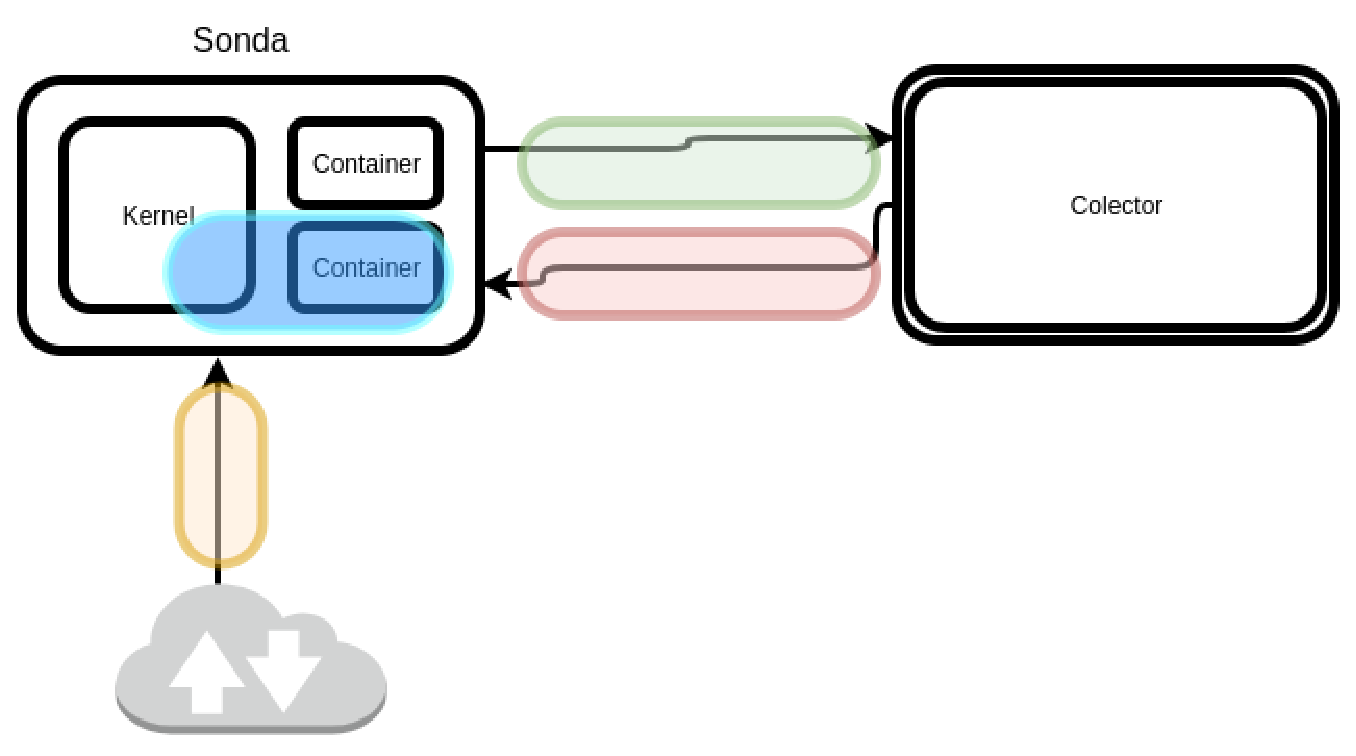
\includegraphics[scale=0.4]{images/threat_model_probe}
  \caption{Modelo de riesgo de la sonda}
  \label{fig:riesgo_sonda}
\end{figure}

Listado de riesgos analizados sobre la figura \ref{fig:riesgo_sonda}:
\begin{enumerate}
    \item[\emph{Naranja 1}] Elevación de privilegios atacando a un servicio expuesto que no pertenece a la \emph{honeypot}. Un atacante puede explotar un servicio de soporte como un servidor SSH de administración o un servicio interno expuesto por mala configuración.
    \item[\emph{Naranja 2}] Riesgo de que la \emph{honeypot} sea reconocible o listada, la \emph{honeypot} es conocida por alguna caracteristica (\emph{IP del servidor, versión del servicio,\ldots}) marcandola como \emph{honeypot} permitiendo a los atacantes simplemente ignorarla.
    \item[\emph{Azul}] El atacante escapa desde el \emph{container}, elevación de privilegios que rompe el aislamiento del kernel y el atacante gana acceso a otros containers o al servidor.
    \item[\emph{Verde}] \emph{Spoofing} de la información enviada al recolector, una vez el atacante gana acceso al servidor puede enviarnos al recolector información falseada.
    \item[\emph{Rojo}] Elevación de privilegios de un atacante que ya ha conseguido acceso al recolector. El recolector y la sonda mantendran una conexión, si alguien ataca al recolector y gana privilegios puede atacar a las sondas. Pese a que es un riesgo, si el recolector ha sido vulnerado, que nos ataquen las sondas no es tan grave.
\end{enumerate}

Listado de mitigaciones para los riesgos analizados:
\begin{enumerate}
    \item[\emph{Naranja 1}] Reducir la superficie de ataque, eliminar servicios expuestos que no pertenezcan a la \emph{honeypot} o limitar el acceso a ciertas direcciones ip conocidas.
    \item[\emph{Naranja 2}] Para mitigar este riesgo, las versiones de las aplicaciones expuestas deben estar ocultas o ser indistinguibles. la mejor alternativa para mitigar éste riesgo es reciclar las sondas, y crear sondas nuevas con suficiente frecuencia. Si el sistema de provisionamiento y configuración de sondas es automatico, se pueden crear nuevas sondas con frecuencia diaria u horaria.
    \item[\emph{Azul}] Debemos aceptar el riesgo, que el container siempre tendra acceso al kernel que se comparte con otros containers y el servidor, como mitigación podemos restringir los privilegios del container para que solo pueda utilizar algunas syscalls, pero en cualquier caso el riesgo de compromiso de un servidor a traves de un container siempre estara presente. 
    \item[\emph{Verde}] La comunicacion entre sonda y recolector se realizara a traves de un canal cifrado con clave asimetrica. En el lado del recolector se pueden realizar validaciones de entrada antes de guardar en base de datos o actuar sobre los eventos recibidos.
    \item[\emph{Rojo}] De todos los riesgos listados, este es el menos grave, si el recolector ha sido atacado y vulnerado tendremos problemas mayores que nuestra sonda sea atacada. La mitigación en este caso es si hemos sido vulnerados cerrar el entorno, apagar los servidores, guardar periodicamente la informacion obtenida en un almacenamiento diferente y externo, hacer una auditoria de seguridad y analisis de que provoco el ataque para repararlo y recrear el entorno desde cero para asegurarnos que el atacante no tiene acceso a el.
\end{enumerate}

Tendremos que tener en cuenta estos riesgos a la hora de modelar la arquitectura y diseñar las protecciones, en general los riesgos \emph{Naranja 1}, \emph{Naranja 2} y \emph{Azul} son mas prioritarios que los riesgos \emph{Verde} y \emph{Rojo}. Las posibles acciones a tomar estan listadas en las mitigaciones del mismo color y creemos que son suficientes para equilibrar los riesgos.

\section{Análisis de soluciones para el recolector}

% 19/08/2017

% % Collector,
%  * registro de las sondas
%  * coleccion de alertas de Falco.
%  * coleccion de trazas del sistema.
%  * Procesamiento de trazas del sistema 
%  * Almacenamiento de informacion


\subsection{registro de las sondas}

El recolector debe conocer el número de sondas desplegadas para poder extraer información de ellas o al menos validar
los eventos que estas envien.

En definitiva debemos preguntarnos como se realizará el registro de sondas y que casos de uso ha de proporcionar. En general, necesitaremos lo siguiente:

\begin{enumerate}
    \item Necesitamos \emph{metadata} de las sondas para la explotación de datos, al menos la ubicación donde la sonda esta desplegada, el proveedor, servicios expuestos en la \emph{honeypot} y versiones.
    \item Como se comentaba en el modelo de seguridad de las sondas, consideramos las sondas como entidades efimeras, que aparecen y desaparecen. 
    Necesitaremos un registro de sondas si queremos realizar analisis historicos, especialmente si queremos permitir el reprocesado de datos.
    \item Verificación de la sonda para mantener la integridad de la información, la sonda ha de identificarse frente al recolector para asegurarnos que la fuente de información es legitima.
    \item De cara a la recolección de datos, tendremos que pensar si optaremos por un modelo \emph{pull} frente a uno \emph{push}. En caso de escoger un modelo \emph{pull} el recolector debe conocer
    cuales son las sondas y su estado para obtener las trazas.
\end{enumerate}

\subsection{Recolección de notificaciones de la \emph{honeypot}}

Las alertas generadas por la \emph{Honeypot} seran eventos en formato textual o binario de un tamaño pequeño ( $<$ 1MiB). 
Es importante que dichos eventos no se pierdan y que sean recolectados con la mayor celeridad posible incluso si las trazas disponibles
y la información de las trazas no está disponible.

Para la recolección de estas notificaciones, tenemos varias opciones, que se listan a continuación.

\subsubsection{Notificaciones a través de HTTP}

La \emph{honeypot} cuando detecta un evento relevante, realiza una petición HTTP a un servicio web de recolección que se ejecuta en el recolector.
Si dicho servicio no está disponible o esta congestionado, el evento se perdera.
La sonda no requiere instalación adicional de \emph{software} ya que sólo requiere realizar una petición HTTP. 
Si la conexión de red de la sonda no funciona al realizar la petición el evento también se perderá.

\subsubsection{Notificaciones usando un sistema de colas}

Tendremos que instalar, configurar y mantener un sistema de colas como \emph{RabbitMQ, ZeroMQ, Kafka} 
o pagar por el uso de sistemas de colas en el \emph{cloud} como \emph{AWS SQS, AWS Kinesis o Google Cloud PubSub}.

La principal ventaja al seguir este enfoque es que los eventos seran almacenados en el sistema de colas y no en las sondas o en el recolector. Si queremos
distribuir las tareas de procesamiento y recolección eventos entre varios recolectores, necesitaremos este elemento central de coordinación.

El principal inconveniente es el coste en terminos economicos y de esfuerzo en mantener esta solucion. 
Si decidimos gestionarlo dentro del proyecto usando algo como \emph{RabbitMQ o Kafka} además del incremento economico en servidores 
debemos añadir el incremento en la complejidad del proyecto. En cambio, si apostamos por utilizar una solución \emph{cloud} la complejidad
de instalación y mantenimiento baja a costa de un mayor desembolso economico y a aceptar las capacidades tecnicas y limites que las soluciones 
\emph{cloud} tienen.

Para este proyecto, el orden estricto de recepción de eventos no es necesario. No nos importará el orden de eventos recibidos siempre y cuando
ningun evento se entregue con demasiada posterioridad.
\begin{table}[h]
    \centering
    \begin{tabular}[!h]{|l|l|r|}
    \hline
    \thead{Opcion} & \thead{Comentarios} & \thead{Coste aproximado} \\
    \hline
    \emph{AWS SQS} & 10.000.000 de peticiones, 3 GiB de transferencia & 5\$ mes \\
    \hline
    \emph{Google PubSub } &  10 GiB de eventos & 0.36\$ mes \\
    \hline
    \emph{RabbitMQ} & 3 instancias (512 MiB,1 CPU, 20 GiB de disco) & 15\$ mes \\
    \hline
    \end{tabular}
    \caption{\label{tab:colas-coste} coste aproximado minimo de sistemas de colas}
    \end{table}


El cuadro \ref{tab:colas-coste} refleja el coste de sistemas actuales con el precio fijado en la fecha de redacción de esta memoria. En el no se contemplan costes indirectos,
como el coste de las horas invertidas en configurar y puesta a punto del sistema, que en el caso de las soluciones \emph{cloud} aunque no es cero, es menor que la solucion de hacerlo \emph{in-house}.

Tampoco se tiene en cuenta la escalabilidad de la solucion, que en el caso de las soluciones \emph{cloud} el sistema es escalable a costa de un precio cada vez mayor, mientras que en la solucion in-house los costes son
fijos hasta que se consuma toda la capacidad. El volumen de eventos a procesar dependera de las condiciones de red de la instalación y el volumen de eventos por lo que no podemos
proporcionar un numero de referencia de eventos a procesar.

Las soluciones \emph{cloud} tienen un coste indirecto, nos ligan a un proveedor en concreto. Si escogemos que nuestras \emph{honeypots} se desplieguen en otros proveedores diferentes, tendremos que hacer
pruebas de red para saber si la conectividad entre proveedores es buena, y tendremos costes adicionales en terminos de trafico de red.

Los proveedores de servicios de computación en exclusiva (\emph{VPS}, \emph{Housing}) no suelen cobrar el trafico de red a no ser que superemos ciertos umbrales.

\subsubsection{Notificaciones usando un recolector de \emph{logs}}

Podemos considerar esta opción como una hibrida de las anteriores, instalaremos una aplicación de recolector de logs en la sonda. 
La sonda escribirá eventos en disco cuando estos se produzcan, el sistema de recoleccion de logs monitorizará los \emph{logs} en disco, y
se encargará de reenviar estos eventos al recolector, preferentemente utilizando un canal seguro para la transmisión.

Si hay problemas en la conectividad de red entre la sonda y el recolector, los eventos se guardarán en un \emph{buffer} en disco y se reenviaran cuando la parte servidor este disponible.

Como ejemplo de estas aplicaciones de recolección de \emph{logs} podemos citar, \emph{rsyslog,logstash,syslog-ng o fluentd}. \emph{rsyslog} y \emph{syslog-ng} son más veteranas, 
en cuanto \emph{logstash} y \emph{fluentd} más recientes. 

La diferencia entre las antiguas y recientes radica en que las recientes hacen enfasis en la capacidad de manipulacion de los \emph{logs} antes de su envio, mientras
que las antiguas estan más probadas y su enfoque es hacia garantizar el envío de \emph{logs} de manera segura.

El coste computacional de estas soluciones aunque no es negligible es muy bajo, es necesario procesar un volumen muy elevado de logs para que tenga impacto.
El recolector deberá encargarse de ser capaz de albergar todos los logs recibidos, ya sea porque a su vez reenvia los \emph{logs} a otra ubicación o se encarga de la 
politica de rotado. 

\subsubsection{Opción escogida}

Para este proyecto escogemos la opción de utilizar un recolector de \emph{logs} en nuestras sondas y reenviarlos a nuestro recolector de eventos. 

\begin{enumerate}
    \item La opción de notificar mediante peticiones HTTP es la más simple desde el punto de vista de la sonda y la deseable, pero no nos otorga garantias de entrega.
    \item Utilizar sistemas de colas es lo deseable para escalar la solución, desacopla los productores de eventos de los consumidores,
     y para la sonda la semantica de entrega es igual de simple que en el caso de la opción HTTP. Sin embargo, el coste economico y la complejidad elevada que introduce no justifica su acogida.
     En un estado posterior del proyecto, siempre se puede pivotar a utilizar un sistema de colas.
\end{enumerate}

En concreto se utilizará \emph{rsyslog} como recolector de \emph{logs} por sus pocas necesidad de memoria y CPU y su estabilidad. Las capacidades de modificación de \emph{logs}
antes de su envio no son necesarias para este proyecto y \emph{logstash} y \emph{fluentd} tienen un \emph{footprint} de uso de memoria mucho mas elevado.

\subsection{recoleccion de trazas}

Las trazas generadas por la \emph{honeypot} seran ficheros binarios de un tamaño elevado ($>$ 25 MiB), en el se recogerán todos los eventos del sistema instrumentalizado (\emph{syscalls},datos,\ldots).
Tendremos que buscar un sistema que nos permita recolectar todas las trazas de todas las sondas. Es importante notar que
las trazas una vez procesadas no son estrictamente necesarias, aunque es útil mantener un historico de ellas por dos motivos:

\begin{enumerate}
    \item Permitir el estudio analitico en base a un historico.
    \item Facilitar el reprocesamiento en caso de errores de procesado (\emph{backfilling}). Idealmente nuestro método de extracción de
    datos deberia ser correcto y tener los suficientes tests y garantias pero aún asi los errores pueden ocurrir.
\end{enumerate}


\subsection{Envio de trazas a almacenamiento en la nube}

Si decidimos no gestionar las trazas nosotros, podemos optar por almacenar las trazas en la nube en soluciones \emph{cloud}. Para conocer el coste aproximado
supongamos que queremos almacenar 500GiB de trazas por mes (aprox 18 GiB por dia). En ese caso, el coste en \emph{AWS} y \emph{Google Cloud} para almacenarlos
en una región europea, teniendo en cuenta los costes de tráfico de salida fuera del proveedor sería:

\begin{table}[h]
    \centering
    \begin{tabular}[!h]{|c|c|}
    \hline
    \thead{Proveedor} & \thead{Coste en dolares} \\
    \hline
    \emph{AWS}, resto de servidores fuera &  57.52 \$ \\
    \hline
    \emph{Google Cloud}, resto de servidores fuera &  78.08 \$ \\
    \hline
    \emph{AWS}, con servidores en mismo proveedor  &  11.89 \$ \\
    \hline
    \emph{Google Cloud}, con servidores en mismo proveedor & 10.44 \$ \\
    \hline
    \end{tabular}
    \caption{\label{tab:almacenamiento-coste} coste aproximado de almacenamiento en la nube para 500 GiB}
    \end{table}

En el cuadro \ref{tab:almacenamiento-coste} se reflejan los costes mensuales de almacenar 500 GiB. En el es sensiblemente más barato si no hay transferencia de datos fuera del proveedor aunque no se incluyen
el coste de estos servidores inicialmente amortizandose el coste de servidores al comprar mayor volumen.

\subsection{Sistema de archivos distribuido}

% GlusterFS

% Ceph
% NFS

\subsection{Envio de trazas a un servidor interno de almacenamiento utilizando \emph{rsyslog}}.

% sistema distribuido de ficheros
% rsyslog 

\subsection{Modelo de datos del recolector}

Almacenamiento infinito (S3 Cloud Storage) vs almacenamiento finito, consecuencias. 

Eleccion de la base de datos, foco en busqueda, modelo time series Fecha -> info, no hay interes a priori de datos historicos
ejemplo del pescado, interesante cuando es reciente, irrelevante cuando ha pasado.

\section{Análisis de soluciones para la API}

% 20/08/2017

\subsection{Objeto de la API}

% consumible por maquinas
% integracion con otras herramientas de seguridad como WAFs, SoCs.

\subsection{Contrato de la API}

% API de consulta, no hay creacion.
% Rate limiting?
% versionada
% Rest vs graphql
% /v1/protocol/incident
% /v1/protocol/incident?from=Date&To=Date&Size
% /v1/protocol/feed
% /v1/protocol/incident.stix



\subsection{versionado}

% Por que versionar

\subsection{Rest}

\subsection{Formatos de representacion}

% JSON, Stix


\section{Resultados finales}

% 25/08/2017

% Arquitectura
%  * Descripcion de la arquitectura.
%  * Registro de las sondas.
%  * securizacion de las sondas.

\subsection{Securizacion de la sonda}

Hay diversas medidas de seguridad a aplicar en la sonda. Si seguimos el principio de defensa en profundidad \cite{wikipedia-defense-in-depth}, aplicaremos diversas capas de proteccion en diferentes sistemas.

\subsubsection{elección del sistema operativo de la sonda}

La eleccion del sistema operativo tiene una componente en la que tendremos que tener en cuenta las capacidades del sistema operativo para su securizacion,
la existencia o no de actualizaciones de seguridad.

Para este proyecto se ha escogido GNU/Linux como sistema operativo por las herramientas que nos provee para gestionar nuestra \emph{honeypot}, 
tendremos que escoger una distribución del sistema operativo que nos provea de actualizaciones de seguridad. 
Se ha escogido Debian como distribución por ser la opción de referencia para servidores y mantener software testado, con actualizaciones de seguridad, \emph{builds} reproducibles y por ser la distribución que más conoce y prefiere el autor, la opción podria haber incluido \emph{CentOS, Container Linux, RHEL \ldots} 

En nuestro caso al escoger \emph{Debian} podremos utilizar el sistema de \emph{unattended-upgrades} para actualizar paquetes del sistema cuando se publiquen actualizaciones de seguridad. Es recomendable seguir
los estandares de la industria, como las guias de securización del \emph{CIS} o del \emph{NIST} (véase \cite{ovh-debian-cis} como ejemplo aplicado), que proporcionan guias de securizacion para la mayoria de distribuciones y que son utilizadas para el cumplimiento de legislación para poder gestionar datos sensibles como tarjeta de credito (PCI-DSS). 

\subsection{Reducción de la superficie de ataque}

\subsection{Configuración del SSH de gestión}


% reduccion de servicios expuestos excepto ssh.
% mover ssh de gestion a otro puerto, y limitar las funciones y accesos.
% configuracion de firewall.

\subsubsection{securizacion del sistema de containers}

% utilizacion de AppArmor
% utilizacion de seccomp
% limitacion de ancho de banda usando TC


%  * Notificacion de nuevas trazas.
% Despliegue
%  * Mantenimiento de la arquitectura usando Ansible.

\section{Planificación}

% 26/08/2017

% Commit inicial 15/2/2016
% Prototipo 21/5/2016
% Construccion de la sonda 21/5/2016 - 20/5/2017
% Construccion del recolector 20/5/2016 - 21/7/2016
% Construccion de la API 21/7/2016 - 22/7/2016

\subsection{Metodologia utilizada: modelo iterativo}
% 27/08/2017

%%% Local Variables: 
%%% mode: latex
%%% TeX-master: "main"
%%% End: